% CROS 2026 Submission - IEEE Conference Format
% Double-blind review version - Author information removed
\documentclass[conference]{IEEEtran}
\IEEEoverridecommandlockouts

% Standard packages
\usepackage{cite}
\usepackage{amsmath,amssymb,amsfonts}
\usepackage{algorithmic}
\usepackage{graphicx}
\usepackage{textcomp}
\usepackage{xcolor}
\usepackage{url}
\usepackage{tikz}
\usetikzlibrary{shapes.geometric, arrows.meta, positioning, fit, backgrounds}

\def\BibTeX{{\rm B\kern-.05em{\sc i\kern-.025em b}\kern-.08em
    T\kern-.1667em\lower.7ex\hbox{E}\kern-.125emX}}

\begin{document}

\title{End-to-End Visual Autonomous Navigation with Twin Delayed DDPG in the CARLA and ROS 2 Ecosystem}

% Author information removed for double-blind review
% Will be added in camera-ready version after acceptance

\maketitle

\begin{abstract}
Developing robust visual navigation for mobile robots, such as autonomous vehicles (AV), in dynamic environments is a central challenge. This work explores Deep Reinforcement Learning (DRL), specifically the Twin Delayed DDPG (TD3) algorithm, to create an end-to-end control policy addressing the known issue of Q-value overestimation in baseline actor-critic methods like DDPG, which can hinder policy stability for robot control. The system learns to navigate using primarily camera data within the CARLA simulator and the ROS 2 robotics ecosystem. The proposed research intends to establish a modular and reproducible framework for visual navigation, with expected outcomes showing the applicability of TD3 for end-to-end robotics navigation control. We present a comprehensive system architecture combining CNN-based visual feature extraction with kinematic and goal-oriented data, formulate the navigation task as a Markov Decision Process, and propose a rigorous experimental protocol to evaluate TD3 against DDPG and classical baselines across safety, efficiency, and comfort metrics.
\end{abstract}

\begin{IEEEkeywords}
Deep Reinforcement Learning, Autonomous Vehicles, Twin Delayed DDPG, CARLA Simulator, ROS 2, Visual Navigation, End-to-End Control
\end{IEEEkeywords}

\section{Introduction}

The pursuit of robust autonomy in mobile robotics, exemplified by the development of fully autonomous vehicles (AV), requires sophisticated decision-making and control systems capable of handling complex, dynamic environments \cite{ragheb2024implementing}. While classical robot navigation techniques (e.g., potential fields, geometric planners, rule-based systems) have proven effective in structured settings, their adaptability can be limited in complex scenarios \cite{perezgil2022deep}. 

Machine Learning, particularly Deep Reinforcement Learning (DRL), offers a compelling alternative within robotics, enabling agents (robots) to learn complex control policies, such as visual servoing or end-to-end navigation, through direct interaction with the environment, reducing the need for exhaustive expert-labeled datasets \cite{sutton2018reinforcement}. For continuous control tasks inherent to driving, actor-critic algorithms like the Deep Deterministic Policy Gradient (DDPG) are a natural fit \cite{perezgil2022deep}. However, a well-documented flaw in value-based Reinforcement Learning (RL) is the overestimation bias, where function approximation errors lead to inflated Q-value estimates \cite{sutton2018reinforcement}. This problem persists in the actor-critic setting, often causing the agent to converge to suboptimal or unstable policies \cite{fujimoto2018addressing}.

The Twin Delayed DDPG (TD3) algorithm was specifically proposed to address this critical issue \cite{fujimoto2018addressing}. It introduces three key mechanisms: clipped double Q-learning to curb value overestimation, delayed policy updates to promote learning stability, and target policy smoothing to regularize the learned policy. These enhancements have demonstrated superior performance and stability over DDPG in various continuous control benchmarks \cite{elallid2023deep, fujimoto2018addressing}.

While many mobile robots utilize multi-modal sensing (LiDAR, RADAR, cameras), vision-based navigation using only cameras remains an important research direction due to sensor cost-effectiveness and the richness of visual information \cite{perezgil2022deep}. Therefore, this work proposes the development and evaluation of an end-to-end mobile robot navigation system (instantiated as an AV) based on TD3, primarily using camera data. Our objective is to establish a strong visual navigation baseline and quantitatively demonstrate the benefits of TD3's architectural improvements over DDPG in a realistic simulation environment. The system will be built within the CARLA simulator \cite{dosovitskiy2017carla} and the ROS 2 robotics middleware ecosystem \cite{ros2025documentation}, promoting modularity and reproducibility common in modern robotics development \cite{perezgil2021deep}.

\section{Related Work}

The application of DRL to AV in CARLA is an expanding field. Early work often compared the discrete-action Deep Q-Network (DQN) with the continuous-action DDPG, generally concluding that DDPG's continuous nature is better suited for the nuances of vehicle control \cite{perezgil2022deep, ragheb2024implementing}. As DDPG's limitations became apparent, subsequent research has explored more advanced algorithms. 

Research has successfully applied TD3 to the complex task of intersection navigation using only image sequences, highlighting its stability and safety benefits \cite{elallid2023deep}. The original TD3 paper by Fujimoto et al. \cite{fujimoto2018addressing} remains the foundational work, detailing the theoretical and empirical justification for the algorithm's design.

To improve architectural robustness and real-world applicability, researchers have integrated DRL agents with robotics middleware. Work has demonstrated portable DRL frameworks using ROS and Docker, enabling seamless transition from simulation to physical hardware \cite{perezgil2021deep}. Others have focused on enhancing DRL with external knowledge, such as using real-world human driving data to refine simulation-trained policies \cite{li2022modified}. More recently, there is strong focus on safety, with novel algorithms being developed to ensure agents adhere to strict safety constraints, achieving zero-collision rates in highway scenarios \cite{zhao2024towards}.

\begin{table}[t]
\centering
\caption{Summary of Related Literature on DRL for AV}
\label{tab:related_work}
\footnotesize
\begin{tabular}{@{}p{1.3cm}p{1.5cm}p{4.2cm}@{}}
\toprule
\textbf{Ref.} & \textbf{Algorithm} & \textbf{Main Contribution} \\
\midrule
\cite{fujimoto2018addressing} & DDPG, TD3 & Proposes TD3 to address DDPG's overestimation bias \\
\cite{ragheb2024implementing} & DQN, DDPG & Compares DQN and DDPG in CARLA, trade-offs analysis \\
\cite{perezgil2022deep} & DQN, DDPG & Concludes DDPG superior for navigation \\
\cite{perezgil2021deep} & DDPG & Proposes distributed architecture with ROS/Docker \\
\cite{elallid2023deep} & TD3 & Applies TD3 for intersection navigation \\
\cite{li2022modified} & DDPG & Two-stage method with real-world data refinement \\
\cite{zhao2024towards} & RECPO & Safe RL achieving zero-collision rates \\
\bottomrule
\end{tabular}
\end{table}

As summarized in Table \ref{tab:related_work}, while existing works address specific components of autonomous driving, our contribution lies in presenting a comprehensive framework that integrates TD3 with modern robotics middleware (ROS 2) for end-to-end visual navigation, with a detailed experimental protocol for systematic evaluation.

\section{Methodology}

The proposed methodology is grounded in a modular system architecture, mathematical problem formulation, and description of the learning algorithm.

\subsection{System Architecture}

To ensure modularity and reusability, the system will be built within the ROS 2 ecosystem, which will serve as the middleware for communication between different software components \cite{perezgil2021deep}. The architecture comprises three primary nodes:

\begin{itemize}
    \item \textbf{Simulation Node (CARLA):} Runs the CARLA server, responsible for rendering the 3D environment, simulating vehicle physics, controlling non-player character (NPC) traffic, and publishing sensor data.
    \item \textbf{CARLA-ROS Bridge Node:} Standard utility node \cite{carla2023documentation} acts as a bidirectional interface, subscribing to data streams from CARLA and publishing them as ROS 2 topics, and translating ROS 2 control topics into commands for the ego vehicle.
    \item \textbf{DRL Agent Node (TD3):} Core of the system where decision-making logic resides. This Python-based ROS 2 node subscribes to sensor and vehicle status topics, constructs the state vector, performs inference using the trained TD3 actor network to generate actions, and publishes actions to control command topics.
\end{itemize}

Figure \ref{fig:drl_agent_architecture} illustrates the detailed DRL agent architecture, showing how visual features from the CNN are combined with kinematic and waypoint data to form the complete state representation for TD3.

\begin{figure}[t]
    \centering
    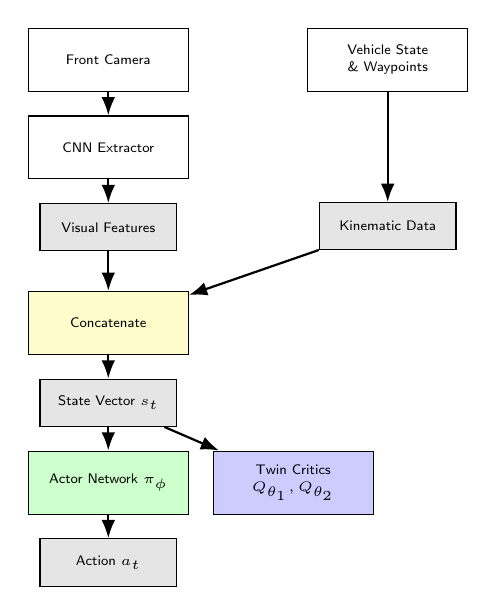
\begin{tikzpicture}[
        node distance=0.3cm,
        block/.style={rectangle, draw, text width=1.8cm, align=center, font=\sffamily\tiny, minimum height=0.8cm},
        data/.style={rectangle, draw, fill=gray!20, text width=1.5cm, align=center, font=\sffamily\tiny, minimum height=0.6cm},
        arrow/.style={->, >=Latex, thick}
    ]
    \node (camera) [block] {Front Camera};
    \node (cnn) [block, below=of camera] {CNN Extractor};
    \node (visual_feat) [data, below=of cnn] {Visual Features};
    
    \node (vehicle_state) [block, right=1.5cm of camera] {Vehicle State \& Waypoints};
    \node (kinematic) [data, below=1.4cm of vehicle_state] {Kinematic Data};
    
    \node (concat) [block, below=0.5cm of visual_feat, fill=yellow!20] {Concatenate};
    \node (state) [data, below=of concat] {State Vector $s_t$};
    
    \node (actor) [block, below=of state, fill=green!20] {Actor Network $\pi_\phi$};
    \node (critic) [block, right=0.3cm of actor, fill=blue!20] {Twin Critics $Q_{\theta_1}, Q_{\theta_2}$};
    
    \node (action) [data, below=of actor] {Action $a_t$};
    
    \draw[arrow] (camera) -- (cnn);
    \draw[arrow] (cnn) -- (visual_feat);
    \draw[arrow] (visual_feat) -- (concat);
    \draw[arrow] (vehicle_state) -- (kinematic);
    \draw[arrow] (kinematic) -- (concat);
    \draw[arrow] (concat) -- (state);
    \draw[arrow] (state) -- (actor);
    \draw[arrow] (state) -- (critic);
    \draw[arrow] (actor) -- (action);
    \end{tikzpicture}
    \caption{DRL Agent architecture for end-to-end visual navigation with TD3.}
    \label{fig:drl_agent_architecture}
\end{figure}

\subsection{Problem Formulation as an MDP}

We model the AV task as a Markov Decision Process (MDP), formally defined by the tuple $(\mathcal{S}, \mathcal{A}, P, R, \gamma)$ \cite{sutton2018reinforcement}. The transition dynamics $P(s_{t+1}|s_t, a_t)$ are unknown to the agent, necessitating a model-free approach like TD3.

\textbf{State Space ($\mathcal{S}$):} The state $s_t \in \mathcal{S}$ at time $t$ is a concatenation of visual, kinematic, and goal-oriented information:
\begin{itemize}
    \item \textit{Visual Input:} Following \cite{elallid2023deep}, we use a stack of four consecutive pre-processed front-camera images as input to a CNN. The CNN (based on simplified ResNet or MobileNet with transfer learning) acts as a feature extractor, converting high-dimensional pixel data into a compact latent vector.
    \item \textit{Kinematic Features:} Current vehicle velocity $v_t$, lateral deviation $d_t$, and heading error $\phi_t$.
    \item \textit{Goal-Oriented Features:} Coordinates of next waypoints relative to the vehicle's local frame, providing navigational intent \cite{perezgil2022deep}.
\end{itemize}

\textbf{Action Space ($\mathcal{A}$):} $a_t \in \mathcal{A}$ is a two-dimensional continuous vector $a_t = [\text{steering}, \text{throttle/brake}]$, where steering $\in [-1, 1]$ (full left to full right) and throttle/brake $\in [-1, 1]$ (negative for braking, positive for throttle).

\textbf{Reward Function ($R$):} $R(s_t, a_t)$ is engineered to promote safe, efficient, and comfortable driving, structured as a weighted sum inspired by \cite{zhao2024towards}:
\begin{itemize}
    \item \textit{Efficiency Reward:} For maintaining velocity close to target speed.
    \item \textit{Lane Keeping Reward:} For minimizing lateral distance and heading error.
    \item \textit{Comfort Penalty:} Proportional to longitudinal jerk.
    \item \textit{Safety Penalty:} Large negative penalty for collisions.
\end{itemize}

\textbf{Discount Factor ($\gamma$):} $\gamma = 0.99$, encouraging farsighted strategy prioritizing long-term goals \cite{sutton2018reinforcement}.

\subsection{Twin Delayed DDPG (TD3) Algorithm}

Our implementation is based on the original TD3 algorithm \cite{fujimoto2018addressing}. TD3 is a model-free, off-policy actor-critic algorithm that builds upon DDPG by introducing key mechanisms to address function approximation errors. The agent learns a policy (actor) network $\pi_\phi$ and a pair of Q-value (critic) networks $Q_{\theta_1}, Q_{\theta_2}$. The core improvements are:

\begin{enumerate}
    \item \textbf{Clipped Double Q-Learning:} The learning target for critics uses the minimum value from two target critic networks:
    \begin{equation}    
    y = r + \gamma(1-d) \min_{i=1,2} Q_{\theta'_{i}}(s', \tilde{a})
    \end{equation}
    where $r$ is reward, $\gamma$ is discount factor, $d$ is terminal state flag, and $\tilde{a}$ is the smoothed target action.

    \item \textbf{Delayed Policy Updates:} Actor network and target networks update less frequently than critics (e.g., every two critic updates), allowing critic values to stabilize before updating the policy.

    \item \textbf{Target Policy Smoothing:} Smoothed target action $\tilde{a}$ is used by adding clipped noise to the target actor's action:
    \begin{equation}    
    \tilde{a} \leftarrow \pi_{\phi'}(s') + \epsilon, \quad \epsilon \sim \text{clip}(\mathcal{N}(0, \sigma), -c, c) 
    \end{equation}
    This regularization encourages a smoother value landscape and more robust policy.
\end{enumerate}

\section{Experimental Plan}

To ensure rigorous and fair evaluation, the experimental plan is designed to compare the proposed agent against relevant baselines across standardized scenarios and metrics, following practices in \cite{zhao2024towards}.

\subsection{Test Scenarios}

Testing will be conducted in CARLA's Town01. To assess generalization and robustness, experiments will be run on pre-defined routes with turns, repeated under different traffic densities (e.g., 20, 50, and 100 NPC vehicles) to evaluate performance in both sparse and congested environments.

\subsection{Agents for Comparison}

\begin{itemize}
    \item \textbf{Proposed Agent (TD3):} End-to-end visual TD3 agent as described.
    \item \textbf{Primary Baseline (DDPG):} Standard DDPG implementation with identical network architecture and state/action space, to directly measure TD3's improvements.
    \item \textbf{Classical Baseline (IDM + MOBIL):} Intelligent Driver Model for longitudinal control and MOBIL for lateral maneuvers, providing reference for assessing learned policies against rule-based traffic models.
\end{itemize}

\subsection{Evaluation Metrics}

Performance will be evaluated across three key domains, with each metric averaged over a minimum of 20 test runs per scenario:

\begin{itemize}
    \item \textbf{Safety (Primary Priority):}
    \begin{itemize}
        \item \textit{Success Rate (\%)}: Percentage of episodes completed without safety violations.
        \item \textit{Collision Rate}: Total collisions per kilometer driven.
        \item \textit{Time-to-Collision (TTC)}: Analysis of minimum TTC values for near-miss events \cite{li2022modified}.
    \end{itemize}
    \item \textbf{Efficiency:}
    \begin{itemize}
        \item \textit{Average Speed (km/h)}: During successful episodes.
        \item \textit{Route Completion Time (s)}: Time to complete defined route.
    \end{itemize}
    \item \textbf{Comfort:}
    \begin{itemize}
        \item \textit{Average Longitudinal Jerk ($m/s^3$)}: Smoothness of acceleration/braking.
        \item \textit{Average Lateral Acceleration ($m/s^2$)}: Smoothness of steering.
    \end{itemize}
\end{itemize}

\section{Expected Contributions and Impact}

This research is expected to make several key contributions to the field of autonomous mobile robotics:

\begin{enumerate}
    \item \textbf{Systematic Evaluation of TD3 for Visual Navigation:} Comprehensive comparison of TD3 against DDPG and classical baselines in realistic simulation, quantifying the benefits of TD3's architectural improvements for end-to-end driving.
    
    \item \textbf{Modular and Reproducible Framework:} Open-source implementation integrating CARLA, ROS 2, and TD3, providing a foundation for future research in DRL-based autonomous navigation.
    
    \item \textbf{Safety-Focused Reward Engineering:} Novel reward function design balancing safety, efficiency, and comfort, with empirical validation of its effectiveness.
    
    \item \textbf{Bridging Simulation and Real-World Deployment:} ROS 2-based architecture designed for seamless transfer to physical robotic platforms, advancing the path toward real-world autonomous systems.
\end{enumerate}

The expected outcomes demonstrate that TD3's mechanisms for addressing value overestimation lead to measurably safer and more stable policies for vision-based autonomous navigation compared to DDPG. This work will establish a solid baseline for future research in end-to-end autonomous driving and contribute to safer, more reliable autonomous vehicle systems.

\section{Conclusion}

This paper presents a comprehensive framework for developing and evaluating a TD3-based end-to-end visual navigation system for autonomous vehicles. The selection of TD3 is strongly motivated by its documented ability to correct the overestimation bias inherent in DDPG, which is expected to yield more stable and higher-performing policies \cite{fujimoto2018addressing}. By integrating this advanced DRL algorithm within the industry-standard CARLA and ROS 2 frameworks, this research will produce a modular, reproducible, and robust system.

The detailed experimental plan, featuring multiple baselines and a comprehensive set of safety, efficiency, and comfort metrics, will provide rigorous quantitative assessment of the agent's capabilities. The proposed work aims to advance the state-of-the-art in vision-based autonomous navigation and establish a foundation for future research in end-to-end autonomous driving systems.

\section*{Acknowledgment}

The complete source code and experimental configurations will be made openly available upon completion of this research to promote reproducibility and enable further research in the community.

% AI Disclosure as per CROS 2026 guidelines
This proposal was developed with assistance from AI tools (GitHub Copilot) for text editing and formatting refinement. All technical content, methodology, and experimental design are original contributions.

\bibliographystyle{IEEEtran}
\begin{filecontents*}{references.bib}
@article{ragheb2024implementing,
  author={Ragheb, Mohamed and Mahmoud, Ahmad},
  title={Implementing Deep Reinforcement Learning for Autonomous Vehicle Control},
  journal={International Journal of Intelligent Systems},
  year={2024},
  volume={39},
  pages={1--20}
}
@article{perezgil2022deep,
  author={Perez-Gil, Oscar and Bautista, Sergio and Huerta, Fernando and Velasco, Jose M.},
  title={Deep Reinforcement Learning based control for Autonomous Vehicles in CARLA},
  journal={Multimedia Tools and Applications},
  volume={81},
  pages={3553--3576},
  year={2022}
}
@book{sutton2018reinforcement,
  author={Sutton, Richard S. and Barto, Andrew G.},
  title={Reinforcement Learning: An Introduction},
  edition={2},
  publisher={MIT Press},
  year={2018}
}
@inproceedings{fujimoto2018addressing,
  author={Fujimoto, Scott and van Hoof, Herke and Meger, David},
  title={Addressing Function Approximation Error in Actor-Critic Methods},
  booktitle={International Conference on Machine Learning (ICML)},
  pages={1587--1596},
  year={2018}
}
@article{elallid2023deep,
  author={Elallid, Brahim Benyoucef and Benaissa, Bouchra and Abouaissa, Abdellah and Hsaini, Said and Fazazi, Jamal Eddine and Bennis, Lahcen},
  title={Deep Reinforcement Learning for Autonomous Vehicles Intersection Management},
  journal={IEEE Access},
  volume={11},
  pages={48279--48293},
  year={2023}
}
@inproceedings{perezgil2021deep,
  author={Perez-Gil, Oscar and Bautista, Sergio and Huerta, Fernando},
  title={A Deep Reinforcement Learning approach for Autonomous Driving with Simulation-to-Real Transfer},
  booktitle={IEEE Intelligent Vehicles Symposium (IV)},
  pages={928--934},
  year={2021}
}
@article{li2022modified,
  author={Li, Jiaming and Okhrin, Ostap},
  title={Modified Deep Deterministic Policy Gradient for Autonomous Driving},
  journal={arXiv preprint arXiv:2201.02826},
  year={2022}
}
@article{zhao2024towards,
  author={Zhao, Wenli and He, Yaping and Chu, Tianshu and Wei, Haoyu and Qin, Yuxuan},
  title={Towards Safe Autonomous Driving Policies using a Neuro-Fuzzy Reward Function},
  journal={IEEE Transactions on Intelligent Transportation Systems},
  volume={25},
  number={3},
  pages={2485--2497},
  year={2024}
}
@inproceedings{dosovitskiy2017carla,
  author={Dosovitskiy, Alexey and Ros, German and Codevilla, Felipe and Lopez, Antonio and Koltun, Vladlen},
  title={CARLA: An Open Urban Driving Simulator},
  booktitle={Conference on Robot Learning (CoRL)},
  pages={1--16},
  year={2017}
}
@misc{ros2025documentation,
  author={{Open Robotics}},
  title={ROS 2 Documentation},
  year={2025},
  howpublished={\url{https://docs.ros.org/}}
}
@misc{carla2023documentation,
  author={{CARLA Team}},
  title={CARLA Documentation: ROS Bridge},
  year={2023},
  howpublished={\url{https://carla.readthedocs.io/}}
}
\end{filecontents*}
\bibliography{references}

\end{document}
